\documentclass[12pt,a4paper]{article}
\usepackage[margin=2.5cm]{geometry}
\usepackage{booktabs}
\usepackage{longtable}
\usepackage{array}
\usepackage{tabularx}
\usepackage{hyperref}
\usepackage{graphicx}
\usepackage{listings}
\usepackage{xcolor}
\usepackage{parskip}
\usepackage{titlesec}
\usepackage{fancyhdr}
\usepackage{caption}
\usepackage{float}
\usepackage{enumitem}
\usepackage{amsmath}

% ── Colours ──────────────────────────────────────────────────────────────────
\definecolor{mongogreen}{RGB}{0,104,74}
\definecolor{neoblue}{RGB}{0,87,166}
\definecolor{codegray}{RGB}{245,245,245}
\definecolor{codeframe}{RGB}{200,200,200}

% ── Code listings ─────────────────────────────────────────────────────────────
\lstdefinestyle{mongo}{
  backgroundcolor=\color{codegray},
  frame=single,
  rulecolor=\color{codeframe},
  basicstyle=\ttfamily\footnotesize,
  breaklines=true,
  breakatwhitespace=true,
  keepspaces=true,
  showstringspaces=false,
  keywordstyle=\color{mongogreen}\bfseries,
  commentstyle=\color{gray},
  stringstyle=\color{neoblue},
  captionpos=b,
  xleftmargin=5pt,
  xrightmargin=5pt,
  aboveskip=6pt,
  belowskip=6pt,
}

\lstdefinestyle{cypher}{
  backgroundcolor=\color{codegray},
  frame=single,
  rulecolor=\color{codeframe},
  basicstyle=\ttfamily\footnotesize,
  breaklines=true,
  breakatwhitespace=true,
  keepspaces=true,
  showstringspaces=false,
  keywordstyle=\color{neoblue}\bfseries,
  commentstyle=\color{gray},
  stringstyle=\color{mongogreen},
  captionpos=b,
  xleftmargin=5pt,
  xrightmargin=5pt,
  aboveskip=6pt,
  belowskip=6pt,
}

% ── Section formatting ────────────────────────────────────────────────────────
\titleformat{\section}{\large\bfseries}{}{0em}{}[\titlerule]
\titleformat{\subsection}{\normalsize\bfseries}{}{0em}{}
\titleformat{\subsubsection}{\normalsize\itshape}{}{0em}{}

% ── Header / Footer ───────────────────────────────────────────────────────────
\pagestyle{fancy}
\fancyhf{}
\lhead{\small CS-3510 Data Science and Management}
\rhead{\small Assignment 2 -- Part 1}
\cfoot{\thepage}
\renewcommand{\headrulewidth}{0.4pt}

% ── Helpers ───────────────────────────────────────────────────────────────────
\newcommand{\code}[1]{\texttt{#1}}
\newcommand{\marks}[1]{\hfill\textit{(#1 marks)}}

% ─────────────────────────────────────────────────────────────────────────────
\begin{document}

% ── Title page ────────────────────────────────────────────────────────────────
\begin{titlepage}
  \centering
  \vspace*{3cm}
  {\Large\bfseries Department of Computer Science\\[0.3em]
  Ashoka University\par}
  \vspace{1.5cm}
  {\LARGE\bfseries CS-3510: Data Science and Management\par}
  \vspace{0.8cm}
  {\Large Assignment 2 -- Part 1\par}
  \vspace{0.5cm}
  {\large NoSQL Database Design and Querying\\with the Yelp Open Dataset\par}
  \vspace{2cm}
  \begin{tabular}{ll}
    \textbf{Name:}        & Agriya Yadav \\[4pt]
    \textbf{email:} & agriya.yadav_ug2023@ashoka.edu.in \\[4pt]
  \end{tabular}
  \vfill
\end{titlepage}

\tableofcontents
\newpage

% ═════════════════════════════════════════════════════════════════════════════
\section{Data Acquisition and MongoDB Schema Design \marks{20}}
% ═════════════════════════════════════════════════════════════════════════════

\subsection{Collection Structure \marks{5}}

The Yelp Open Dataset was subsetted by filtering for five major U.S.\ cities:
\textbf{Philadelphia, Tucson, Tampa, Indianapolis, and Nashville}. These cities
were selected to represent geographic diversity across the United States and to
provide non-trivial data volumes while remaining computationally manageable.
The city-based subsetting strategy ensures that all related entities
(businesses, reviews, users, tips, checkins) remain interconnected, which is
critical for both MongoDB aggregation pipelines and Neo4j graph traversals.

The MongoDB database (\code{yelp\_db}) is organised into \textbf{four
collections}:

\begin{table}[H]
  \centering
  \begin{tabular}{lrl}
    \toprule
    \textbf{Collection} & \textbf{Records} & \textbf{Source File(s)} \\
    \midrule
    \code{businesses} & 47,380   & \code{business.json} + \code{checkin.json} (embedded) \\
    \code{users}      & 819,169  & \code{user.json} \\
    \code{reviews}    & 2,640,381 & \code{review.json} \\
    \code{tips}       & 347,238  & \code{tip.json} \\
    \bottomrule
  \end{tabular}
  \caption{MongoDB collections in \code{yelp\_db}}
\end{table}

The source dataset contains six JSON files, but only four were mapped to
collections. \textbf{Checkins} were embedded directly into business documents
(as an array of date strings) rather than kept as a standalone collection.
\textbf{Photos} (\code{photo.json}) were excluded entirely because no
analytical query in this assignment requires photo data, and including them
would add storage overhead without value.

\subsection{Collection Descriptions \marks{5}}

\textbf{\code{businesses}} --- The core entity collection. Each document is
identified by \code{business\_id} (unique index) and contains \code{name},
\code{city}, \code{state}, \code{stars}, \code{review\_count},
\code{address}, \code{latitude}, \code{longitude}, and \code{is\_open}.
The \code{categories} field stores a comma-separated string of business
categories. Two nested sub-documents --- \code{attributes} (e.g., WiFi,
parking, price range) and \code{hours} (operating hours by day of week) ---
are embedded directly. The \code{checkins} field is an embedded array of
ISO-formatted date strings sourced from \code{checkin.json}. This collection
is referenced by \code{reviews} and \code{tips} via \code{business\_id}.

\textbf{\code{users}} --- Stores Yelp user account data. Each document is
identified by \code{user\_id} (unique index) and includes \code{name},
\code{review\_count}, \code{yelping\_since}, engagement metrics (\code{useful},
\code{funny}, \code{cool} vote counts), \code{elite} status, \code{average\_stars},
\code{fans}, and various compliment counters. The \code{friends} field is an
array of \code{user\_id} strings --- a self-referential reference list pointing
to other documents in the same collection.

\textbf{\code{reviews}} --- Contains user-written reviews. Each document is
identified by \code{review\_id} and includes \code{user\_id} and
\code{business\_id} (cross-collection foreign keys), \code{stars}
(1--5 integer), vote counts (\code{useful}, \code{funny}, \code{cool}), full
review \code{text}, and \code{date}. This is the largest collection and serves
as the primary analytical join point between users and businesses.

\textbf{\code{tips}} --- Stores short-form user tips without star ratings.
The combination of \code{user\_id}, \code{business\_id}, and \code{date} serves
as a compound key. Includes \code{text} and \code{compliment\_count}. References
both \code{users} and \code{businesses} via their respective ID fields.

\subsection{Schema Justifications \marks{10}}

\subsubsection{(a) Embed vs.\ Reference Decisions}

\begin{longtable}{>{\bfseries}p{3.2cm}p{2.2cm}p{8.6cm}}
  \toprule
  Relationship & Decision & Justification \\
  \midrule
  \endhead
  Business $\leftrightarrow$ Checkins
    & Embedded
    & Checkins have no independent existence --- they are never queried
      separately from their business. Every analytical use (Query 7) accesses
      them alongside the business document. The data is bounded: each checkin
      is just a date string. Embedding enables single-document reads without
      joins. \\[6pt]
  Business $\leftrightarrow$ Attributes/Hours
    & Embedded (sub-docs)
    & Descriptive metadata belonging exclusively to one business, always
      accessed as part of that document, never queried independently. They
      naturally map to nested objects. \\[6pt]
  User $\rightarrow$ Friends
    & Array of references
    & Friends are full User entities with large documents. Duplicating entire
      user documents inside each friend list would create massive redundancy
      and risk exceeding the 16\,MB document limit for well-connected users.
      Storing an array of \code{user\_id} strings keeps the user document lean
      while enabling friend-count analytics via \code{\$size}. \\[6pt]
  Review $\rightarrow$ Business/User
    & Cross-collection reference
    & Reviews are large (text averages $\sim$550 chars) and grow unboundedly.
      Embedding them into business documents would make those documents
      enormous and eventually exceed the 16\,MB limit. Reviews are also
      independently queried (filtered by date, grouped by user). A separate
      collection with indexed foreign keys is the right model. \\[6pt]
  Tip $\rightarrow$ Business/User
    & Cross-collection reference
    & Same reasoning as reviews: tips grow unboundedly per business and are
      queried independently. \\
  \bottomrule
\end{longtable}

\subsubsection{(b) Read/Write Trade-offs}

\textbf{Embedding checkins} --- \textit{Read trade-off}: Positive. Loading a
business document automatically loads its entire check-in history in a single
fetch. Query 7 (\code{\$size} on the \code{checkins} array) runs as a
single-collection aggregation with no joins required. \textit{Write trade-off}:
Slight negative. Every new check-in appends to the array and re-writes the
document. However, since the Yelp dataset is a static analytical dataset (no
live writes), the read benefit decisively wins.

\textbf{Referencing reviews} --- \textit{Read trade-off}: Negative. Queries
that need both review content and business details (Queries 2, 4) require a
\code{\$lookup} stage, incurring additional I/O. \textit{Write trade-off}:
Positive. New reviews are inserted as standalone documents without touching
the business document at all --- no re-writes, no array growth.

\textbf{Referencing friends} --- \textit{Read trade-off}: Negative for
friend-detail queries (must resolve each \code{user\_id} to fetch friend
profiles), but positive for friend-count queries (\code{\$size} is O(1)).
\textit{Write trade-off}: Moderate negative. Adding/removing a friend requires
updating the \code{friends} array on both user documents. However, no MongoDB
query in this assignment requires friend-detail resolution --- social graph
analysis is delegated to Neo4j.

\subsubsection{(c) Indexes}

Six separate indexes were defined (exceeding the minimum requirement of four)
to optimise the specific queries outlined in Section~5.

\begin{table}[H]
  \centering
  \begin{tabularx}{\textwidth}{llll>{\raggedright\arraybackslash}X}
    \toprule
    \textbf{Field} & \textbf{Collection} & \textbf{Type} & \textbf{Query(s)} & \textbf{Justification} \\
    \midrule
    \code{business\_id} & \code{businesses} & Unique & 2, 4, 7 & Foreign key join target for \code{\$lookup} from \code{reviews}. Without this, every join scans 47K documents. \\[4pt]
    \code{city}         & \code{businesses} & Standard & 1, 2 & Enables efficient grouping by city and city+year. \\[4pt]
    \code{stars}        & \code{businesses} & Standard & 1, 3 & Supports range-based bucketing and sorting. \\[4pt]
    \code{user\_id}     & \code{users}      & Unique & 6 & \code{\$lookup} from \code{reviews} into \code{users}. O(log n) over 819K documents. \\[4pt]
    \code{business\_id} & \code{reviews}    & Standard & 2, 4 & Every review aggregation that joins to businesses uses this. \\[4pt]
    \code{user\_id}     & \code{reviews}    & Standard & 6 & Join from reviews to users over 2.6M documents. \\
    \bottomrule
  \end{tabularx}
  \caption{Indexes defined in \code{yelp\_db}}
\end{table}

% ═════════════════════════════════════════════════════════════════════════════
\section{Entity-Relationship (E-R) Diagram \marks{8}}
% ═════════════════════════════════════════════════════════════════════════════

\begin{figure}[H]
  \centering
  \includegraphics[width=\textwidth]{../ER_Diagram.png}
  \caption{Entity-Relationship diagram for the MongoDB model}
\end{figure}

The E-R diagram represents the four MongoDB collections as entities. Key
features:

\begin{itemize}
  \item \textbf{BUSINESS $\leftrightarrow$ CHECKIN}: Shown with an
    \textit{embedded} relationship (double-bordered / labelled connection).
    Checkins are not a separate collection --- they exist as an array within
    each business document. This is visually distinguished from
    cross-collection references to emphasise the modelling choice.

  \item \textbf{REVIEW $\rightarrow$ BUSINESS} and
    \textbf{REVIEW $\rightarrow$ USER}: Standard relationship lines with FK
    labels indicating cross-collection references via \code{business\_id} and
    \code{user\_id}. Reviews form the primary many-to-many junction between
    users and businesses.

  \item \textbf{TIP $\rightarrow$ BUSINESS} and \textbf{TIP $\rightarrow$ USER}:
    Same referencing pattern as reviews. Tips connect users to businesses
    without star ratings.

  \item \textbf{USER $\leftrightarrow$ USER (friends\_with)}: A
    self-referential relationship represented by a looping arrow. This models
    the \code{friends} array --- an array of \code{user\_id} references
    pointing to other documents in the same \code{users} collection. This is
    not an embedding; it is an array of foreign key references.
\end{itemize}

The distinction between embedded and referenced relationships mirrors the
schema design decisions justified in Section~1.3(a). Checkins are embedded
because they are bounded and always co-accessed with their business. Reviews
and tips are referenced because they grow unboundedly and are independently
queried.

% ═════════════════════════════════════════════════════════════════════════════
\section{Document Schema Diagram \marks{7}}
% ═════════════════════════════════════════════════════════════════════════════

\begin{figure}[H]
  \centering
  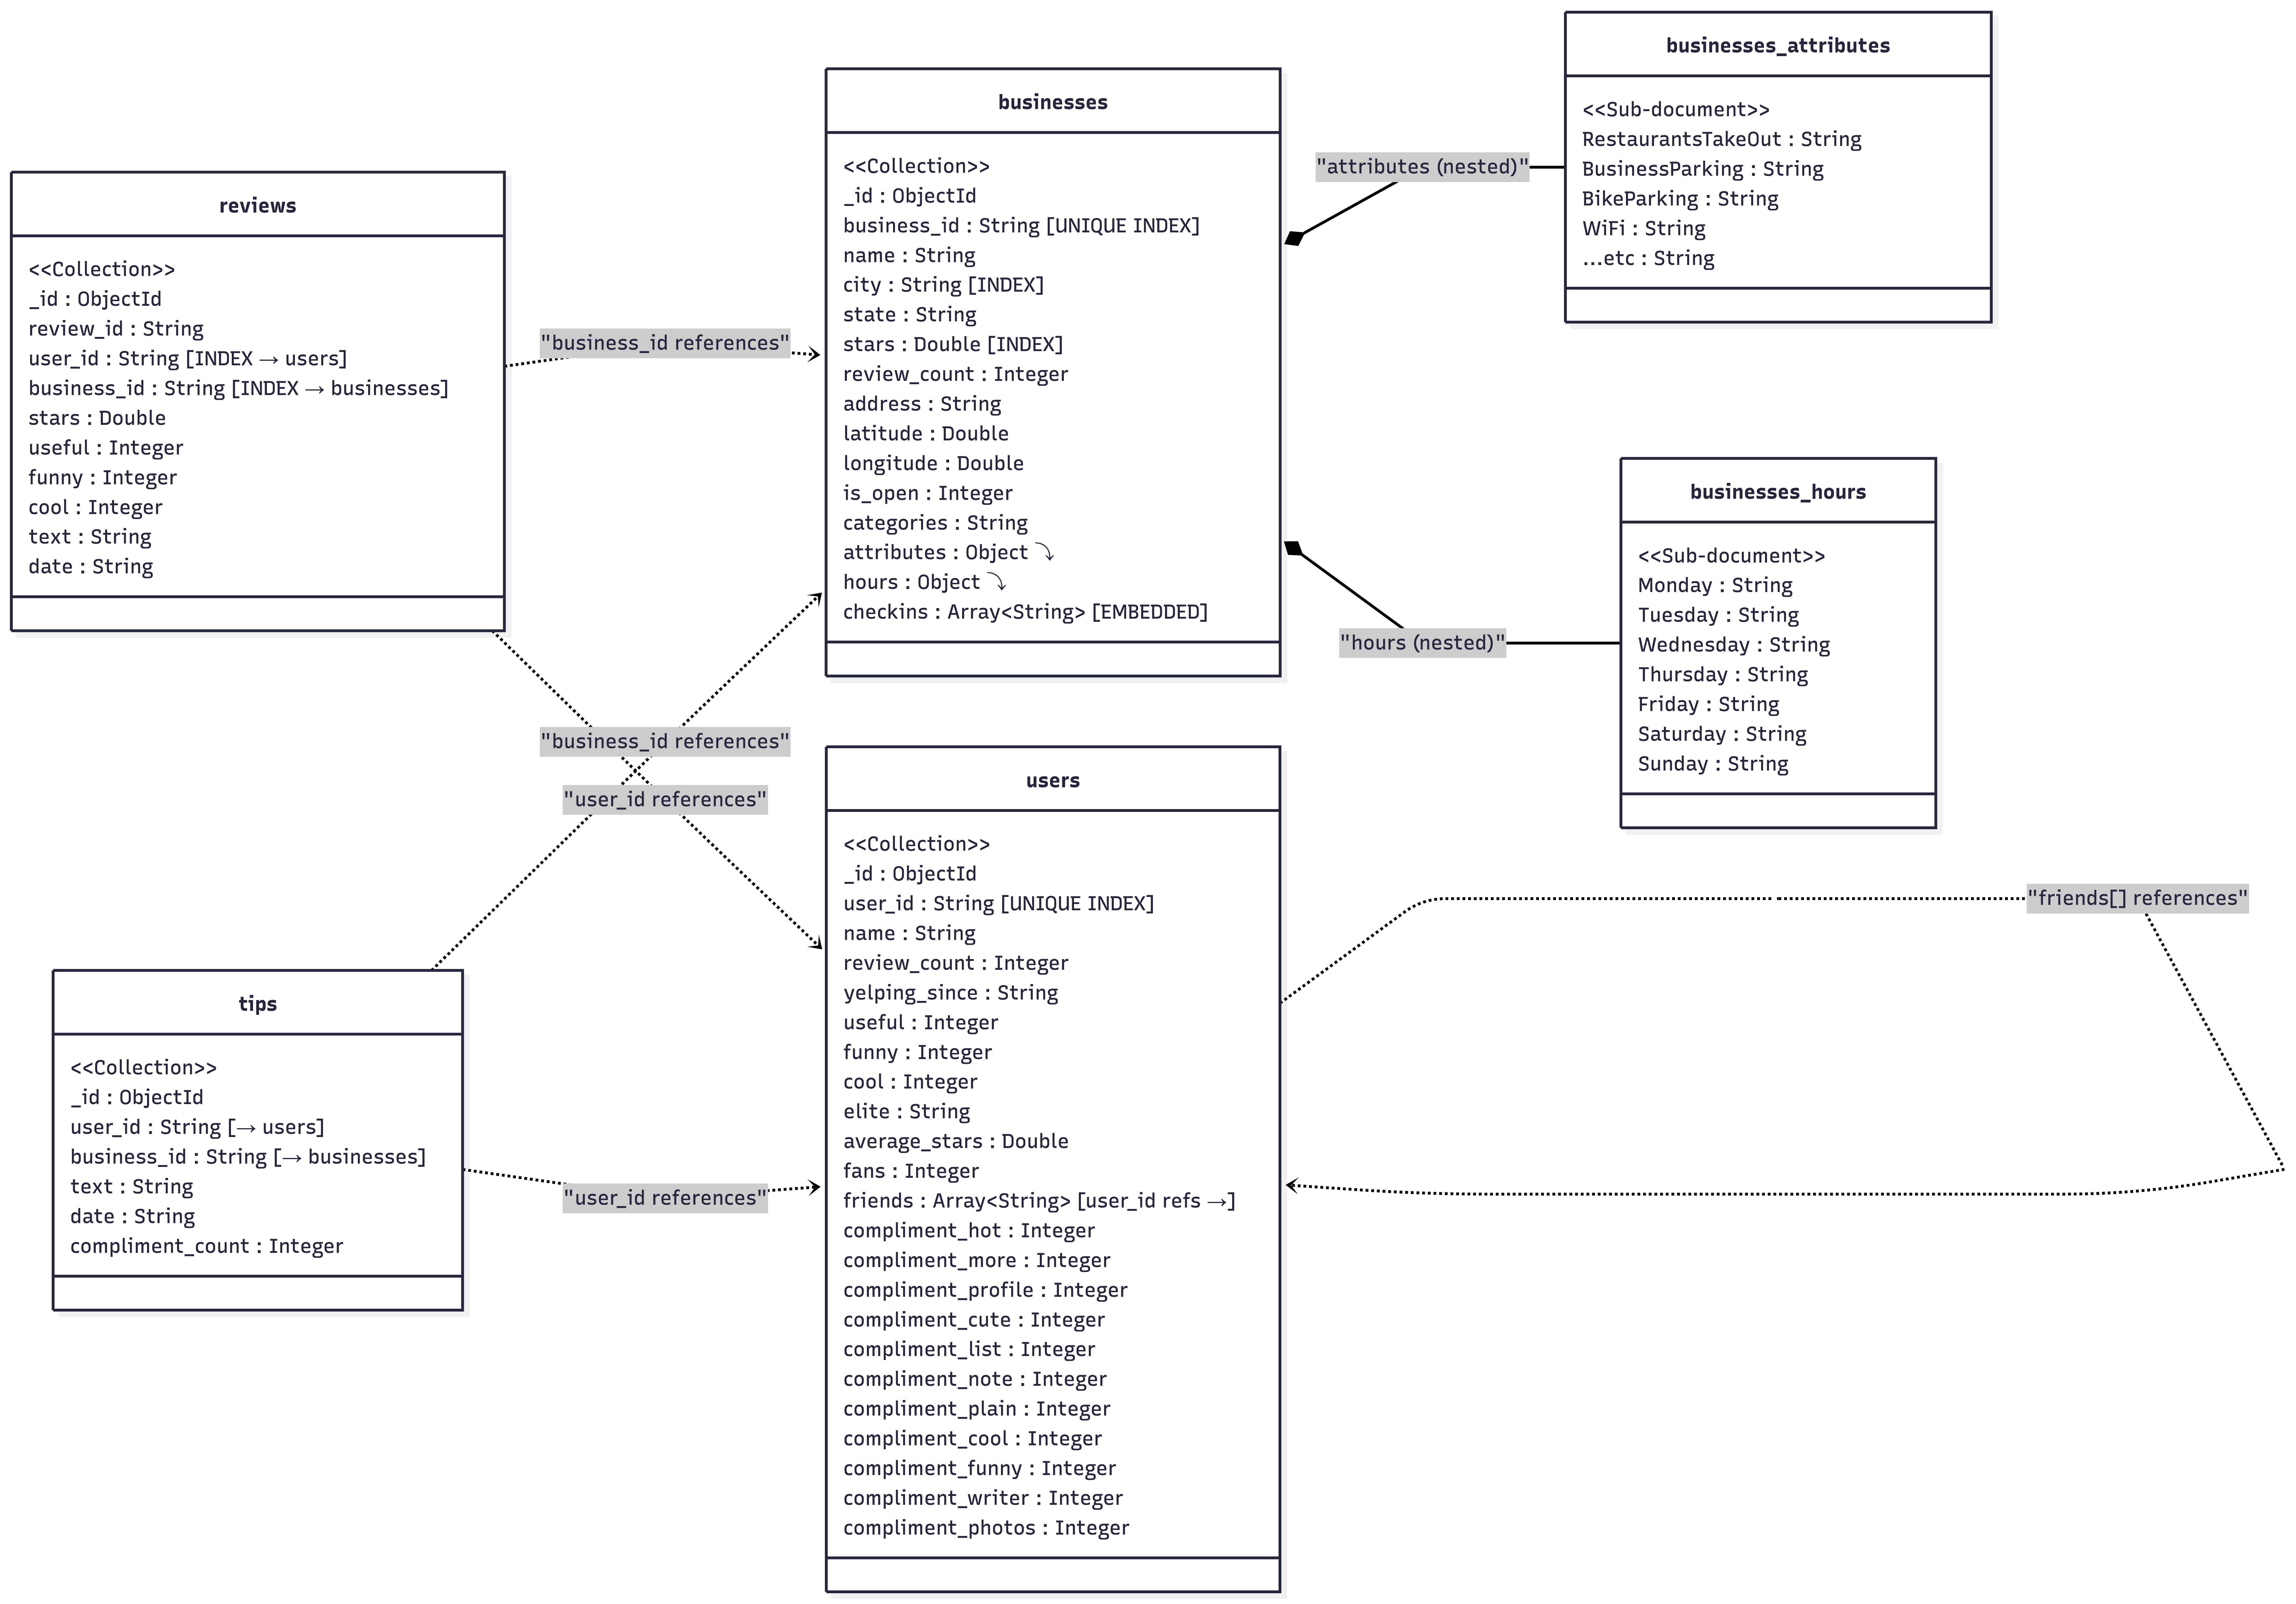
\includegraphics[width=\textwidth]{../classDiagram.png}
  \caption{Document schema diagram showing collection structure, fields, types, and references}
\end{figure}

The document schema diagram shows the internal structure of each collection ---
fields, data types, nested sub-documents, and cross-collection references.

\begin{itemize}
  \item \textbf{\code{businesses.checkins: Array<String>}} --- Labelled as
    EMBEDDED. This array of date strings was sourced from \code{checkin.json}
    and merged into business documents during ingestion. The diagram shows it
    as an internal array, not a separate entity.

  \item \textbf{\code{businesses.attributes} and \code{businesses.hours}} ---
    Shown as nested sub-documents (child classes connected with composition
    arrows). \code{attributes} contains variable key-value pairs (e.g.,
    \code{RestaurantsTakeOut}, \code{WiFi}, \code{BikeParking}), while
    \code{hours} contains day-of-week strings. These are objects nested within
    the business document, not separate collections.

  \item \textbf{\code{users.friends: Array<user\_id refs>}} --- Shown as an
    array field with a reference arrow pointing back to the \code{users}
    collection. Friend data is not embedded user documents --- it is an array
    of string references.

  \item \textbf{\code{reviews.business\_id [INDEX]} and
    \code{reviews.user\_id [INDEX]}} --- Shown with reference arrows pointing
    to \code{businesses} and \code{users} respectively, labelled with INDEX to
    indicate both fields are indexed for efficient \code{\$lookup} joins.

  \item \textbf{Index annotations} are marked directly on fields:
    \code{businesses.business\_id [UNIQUE INDEX]}, \code{businesses.city
    [INDEX]}, \code{businesses.stars [INDEX]}, \code{users.user\_id [UNIQUE
    INDEX]}, \code{reviews.business\_id [INDEX]}, \code{reviews.user\_id
    [INDEX]}.
\end{itemize}

% ═════════════════════════════════════════════════════════════════════════════
\section{Neo4j Property Graph Model \marks{8}}
% ═════════════════════════════════════════════════════════════════════════════

\begin{figure}[H]
  \centering
  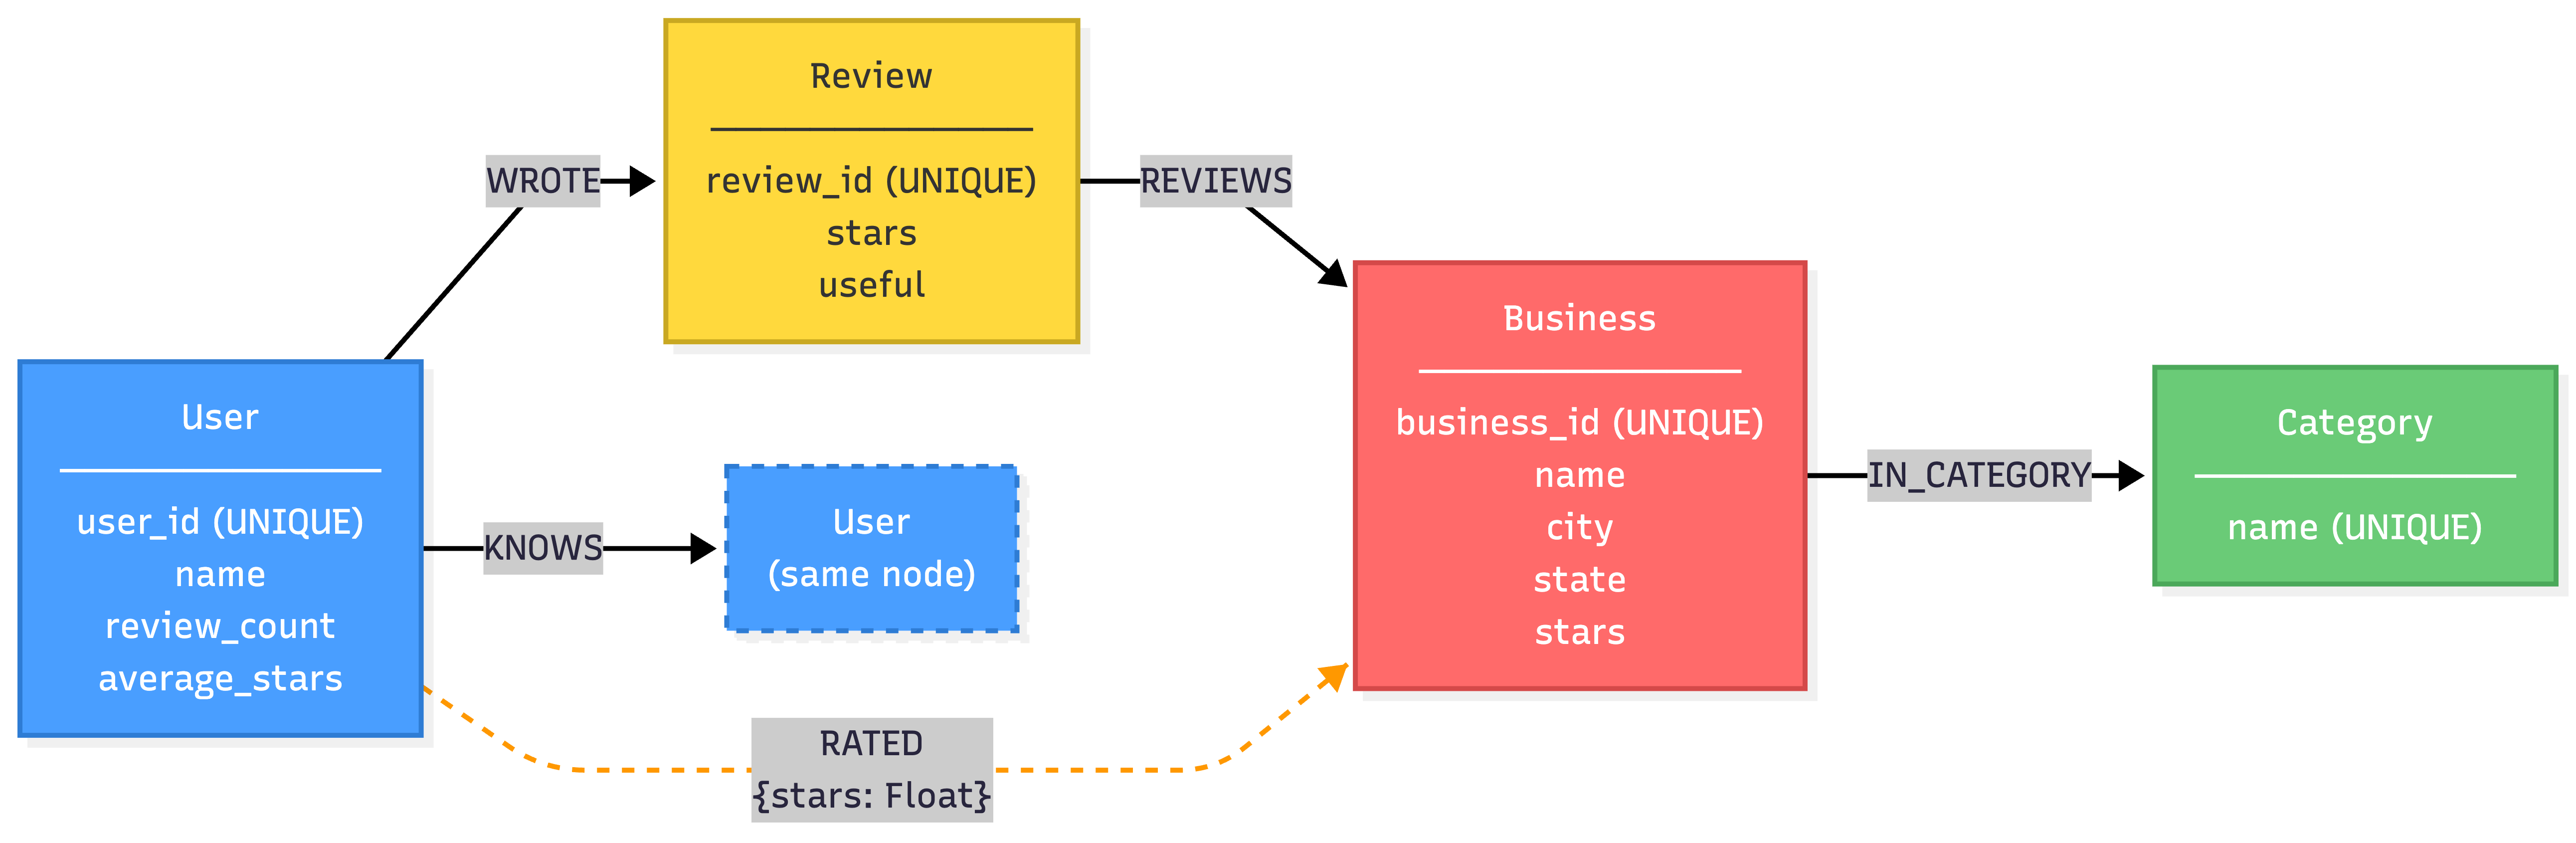
\includegraphics[width=\textwidth]{../graphDiagram.png}
  \caption{Neo4j property graph model diagram}
\end{figure}

\subsection*{Node Labels and Properties}

\begin{table}[H]
  \centering
  \begin{tabular}{lll}
    \toprule
    \textbf{Node Label} & \textbf{Properties} & \textbf{Constraint} \\
    \midrule
    \code{:User}     & \code{user\_id}, \code{name}, \code{review\_count}, \code{average\_stars} & \code{user\_id} UNIQUE \\
    \code{:Business} & \code{business\_id}, \code{name}, \code{city}, \code{state}, \code{stars} & \code{business\_id} UNIQUE \\
    \code{:Review}   & \code{review\_id}, \code{stars}, \code{useful} & \code{review\_id} UNIQUE \\
    \code{:Category} & \code{name} & \code{name} UNIQUE \\
    \bottomrule
  \end{tabular}
\end{table}

\subsection*{Relationship Types}

\begin{table}[H]
  \centering
  \begin{tabularx}{\textwidth}{llll>{\raggedright\arraybackslash}X}
    \toprule
    \textbf{Relationship} & \textbf{From} & \textbf{To} & \textbf{Properties} & \textbf{Description} \\
    \midrule
    \code{WROTE}       & User     & Review   & ---              & User authored a review \\
    \code{REVIEWS}     & Review   & Business & ---              & Review is about a business \\
    \code{RATED}       & User     & Business & \code{stars: Float} & Shortcut denormalization edge \\
    \code{IN\_CATEGORY} & Business & Category & ---              & Business belongs to a category \\
    \code{KNOWS}       & User     & User     & ---              & Social friendship (self-referential) \\
    \bottomrule
  \end{tabularx}
\end{table}

\subsection*{Modelling Choices}

\textbf{Review as a node, not an edge}: Reviews carry rich properties
(\code{stars}, \code{useful}) and sit between two entity types. Modelling
Review as a node allows properties to be attached naturally and enables
flexible multi-hop traversal patterns. If reviews were edges, attaching
multiple properties would be less clean.

\textbf{RATED shortcut relationship}: The \code{RATED} edge is a denormalized
shortcut from User directly to Business, storing the \code{stars} property.
This avoids the two-hop traversal
\code{(User)-[:WROTE]->(Review)-[:REVIEWS]->(Business)} for common queries.
The trade-off is slight storage redundancy.

\textbf{Category as a separate node}: In MongoDB, categories are stored as a
comma-separated string requiring \code{\$split} and \code{\$unwind} for
analysis. In Neo4j, each category is a separate node with \code{IN\_CATEGORY}
edges, naturally handling the many-to-many relationship as simple edge
traversal.

\textbf{KNOWS relationship (directed)}: The source data provides one direction
(user A lists user B as a friend), so edges are directed. Cypher queries
account for this by matching outgoing edges \code{(u)-[:KNOWS]->(f)}.

\subsection*{Data That Does Not Map Naturally to a Graph}

\begin{itemize}
  \item \textbf{Checkins} --- A time-series list of timestamps. Graphs do not
    have a natural ordered sequence structure; modelling each checkin as a node
    would create millions of nodes with minimal traversal value. Handled as the
    embedded array in MongoDB.

  \item \textbf{Business attributes/hours} --- A sparse, schema-less key-value
    set. Graph nodes expect consistent property sets. These were left out of
    the graph model.

  \item \textbf{Review text} --- Free-text has no graph traversal value.
    Excluded from Review nodes to keep the graph lightweight. Text analysis is
    performed in MongoDB.
\end{itemize}

% ═════════════════════════════════════════════════════════════════════════════
\section{MongoDB Queries \marks{20}}
% ═════════════════════════════════════════════════════════════════════════════

\subsection{Query 1: Safest and Least-Safe Cities and Business Categories \marks{2}}

\subsubsection*{Part A --- By City (businesses with $\geq$20 reviews)}

\begin{table}[H]
  \centering
  \begin{tabular}{lrrl}
    \toprule
    \textbf{City} & \textbf{Avg Stars} & \textbf{Total Reviews} & \textbf{Business Count} \\
    \midrule
    Philadelphia  & 3.69 & 863,550 & 7,148 \\
    Indianapolis  & 3.66 & 307,878 & 3,257 \\
    Nashville     & 3.65 & 405,627 & 3,355 \\
    Tampa         & 3.63 & 390,233 & 3,909 \\
    Tucson        & 3.59 & 335,105 & 3,853 \\
    \bottomrule
  \end{tabular}
\end{table}

Philadelphia leads at 3.69 average stars; Tucson ranks lowest at 3.59. The
narrow range (0.10 stars) indicates all five cities are generally well-rated.
The \code{\$match: \{ review\_count: \{ \$gte: 20 \} \}} filter ensures
statistical significance by excluding businesses with too few reviews.

\subsubsection*{Part B --- By Category (top 5 safest and least-safe)}

\begin{table}[H]
  \centering
  \begin{tabular}{clcl}
    \toprule
    \textbf{Rank} & \textbf{Safest Categories} & \textbf{Avg Stars} \\
    \midrule
    1 & Barre Classes           & 4.71 \\
    2 & Home Window Tinting     & 4.63 \\
    3 & Challenge Courses       & 4.61 \\
    4 & Event Photography       & 4.61 \\
    5 & Dog Walkers             & 4.60 \\
    \bottomrule
  \end{tabular}
  \quad
  \begin{tabular}{clc}
    \toprule
    \textbf{Rank} & \textbf{Least-Safe Categories} & \textbf{Avg Stars} \\
    \midrule
    1 & Television Service Providers & 1.63 \\
    2 & Utilities                    & 1.77 \\
    3 & Internet Service Providers   & 1.94 \\
    4 & Truck Rental                 & 2.18 \\
    5 & Banks \& Credit Unions       & 2.20 \\
    \bottomrule
  \end{tabular}
  \caption{Top and bottom categories by average star rating}
\end{table}

The highest-rated categories are niche, passion-driven services (fitness,
photography, pet care) where customers self-select and providers are
intrinsically motivated. The lowest-rated categories are utility/necessity
services (telecom, banking, truck rental) --- industries where customers have
little choice and friction is inherent to the service model.

\subsection{Query 2: Star Rating Trends Over Time \marks{3}}

\subsubsection*{Part A --- City Trends}

The aggregation joins reviews with businesses to extract year and city, then
computes average ratings per city-year combination.

\begin{itemize}
  \item \textbf{Early years (2005--2007)}: Inflated ratings (3.9--4.7) due to
    very few reviews --- enthusiastic early adopters creating positive selection
    bias.
  \item \textbf{Stabilisation (2010--2019)}: Ratings converge around 3.7--3.9
    as review volume grows into tens of thousands per city per year.
  \item \textbf{COVID year (2020)}: Review counts drop sharply (Indianapolis:
    50,236 in 2019 $\to$ 30,620 in 2020) but average ratings increase slightly
    (3.83 $\to$ 3.91). People only visited places they trusted during lockdowns.
  \item \textbf{2022 truncation}: Counts dramatically lower (Indianapolis: 1,829
    vs 34,140 in 2021) --- the dataset ends mid-year.
\end{itemize}

\subsubsection*{Part B --- Category Trends (early 3 years vs.\ late 3 years)}

\begin{table}[H]
  \centering
  \begin{tabular}{lccr}
    \toprule
    \textbf{Category} & \textbf{Early Avg} & \textbf{Late Avg} & \textbf{Change} \\
    \midrule
    \multicolumn{4}{l}{\textit{Strongest upward trends}} \\
    Tiki Bars          & 3.30 & 4.12 & +0.81 \\
    Limos              & 3.04 & 3.74 & +0.70 \\
    Home Cleaning      & 3.19 & 3.86 & +0.67 \\
    Tea Rooms          & 3.77 & 4.41 & +0.64 \\
    Beaches            & 3.54 & 4.18 & +0.63 \\
    \midrule
    \multicolumn{4}{l}{\textit{Strongest downward trends}} \\
    Hospitals          & 3.46 & 2.40 & $-$1.06 \\
    Walk-in Clinics    & 3.76 & 2.71 & $-$1.04 \\
    Banks \& Credit Unions & 3.10 & 2.07 & $-$1.03 \\
    Car Rental         & 3.04 & 2.19 & $-$0.85 \\
    Packing Supplies   & 3.83 & 2.98 & $-$0.84 \\
    \bottomrule
  \end{tabular}
  \caption{Category rating trends (early vs.\ late years)}
\end{table}

Experiential categories (Tiki Bars, Limos, Tea Rooms) trend upward as
standards improved over time. Healthcare and essential services (Hospitals,
Banks, Car Rental) trend sharply downward --- as Yelp's user base grew,
platforms increasingly became outlets for venting systemic service frustrations.

\subsection{Query 3: Review Volume vs.\ Average Star Rating \marks{2}}

\begin{table}[H]
  \centering
  \begin{tabular}{lrr}
    \toprule
    \textbf{Review Count Bucket} & \textbf{Avg Stars} & \textbf{Business Count} \\
    \midrule
    0--9      & 3.59 & 14,608 \\
    10--49    & 3.55 & 21,986 \\
    50--99    & 3.66 &  4,980 \\
    100--499  & 3.79 &  5,181 \\
    500--999  & 3.97 &    489 \\
    1000--4999 & 4.07 &   134 \\
    5000+     & 4.50 &      2 \\
    \bottomrule
  \end{tabular}
\end{table}

There is a clear \textbf{positive correlation}: businesses with more reviews
tend to have higher average ratings. This is explained by \textbf{survivorship
bias} --- poorly-rated businesses close, so only high-quality businesses
accumulate large review counts. \textit{Practical implication}: raw star
ratings should always be contextualised with review count.

\subsection{Query 4: Review Behaviour Across Business Categories \marks{4}}

\begin{table}[H]
  \centering
  \begin{tabular}{lrrrr}
    \toprule
    \textbf{Category} & \textbf{Avg Stars} & \textbf{Avg Useful} & \textbf{Avg Text (chars)} & \textbf{Total Reviews} \\
    \midrule
    Counseling \& Mental Health & 3.06 & 4.52 & 906  & 1,370 \\
    Lawyers                     & 3.39 & 4.51 & 575  & 1,809 \\
    Insurance                   & 2.71 & 3.87 & 642  & 2,497 \\
    Colleges \& Universities    & 3.21 & 3.79 & 838  & 1,913 \\
    Property Management         & 2.53 & 3.46 & 877  & 6,243 \\
    Apartments                  & 2.67 & 2.86 & 961  & 15,548 \\
    \bottomrule
  \end{tabular}
\end{table}

\textbf{Counseling \& Mental Health} and \textbf{Lawyers} top the useful-votes
ranking --- high-stakes categories where readers seek detailed guidance before
making decisions. These same categories have the longest reviews (906 and 838
avg chars). \textbf{Low-rated categories} (Insurance 2.71, Apartments 2.67,
Property Management 2.53) reflect structural dissatisfaction --- services
people use out of necessity, not choice. The negative sentiment is systemic,
not business-specific.

\subsection{Query 5: Impact of User Tenure on Reviewing Behaviour \marks{3}}

\begin{table}[H]
  \centering
  \begin{tabular}{lrrr}
    \toprule
    \textbf{Tenure (years)} & \textbf{Avg Stars} & \textbf{Avg Useful Votes} & \textbf{Total Users} \\
    \midrule
    0--1  & 2.79 & 0.16   &    908 \\
    2--4  & 3.30 & 4.24   & 72,811 \\
    5--9  & 3.65 & 22.49  & 401,631 \\
    10--14 & 3.74 & 91.39 & 321,286 \\
    15+   & 3.76 & 431.73 &  22,533 \\
    \bottomrule
  \end{tabular}
\end{table}

Useful votes increase \textbf{2,700$\times$} from the 0--1 year cohort to the
15+ year cohort (0.16 $\to$ 431.73). Veteran users contribute
disproportionately to platform value despite being a small minority. Stars
increase slightly with tenure (2.79 $\to$ 3.76) --- newer users give extreme
ratings; experienced users calibrate more moderately over time.

\subsection{Query 6: Elite vs.\ Non-Elite Users \marks{3}}

\begin{table}[H]
  \centering
  \begin{tabular}{lrrr}
    \toprule
    \textbf{Metric} & \textbf{Non-Elite} & \textbf{Elite} & \textbf{Difference} \\
    \midrule
    Mean star rating given          & 3.70 & 3.98 & +0.28 \\
    Mean review character length    & 507  & 780  & +54\% \\
    Mean useful votes per review    & 0.82 & 2.11 & +2.6$\times$ \\
    Total reviews                   & 1,874,725 & 765,646 & --- \\
    \bottomrule
  \end{tabular}
\end{table}

Elite users write \textbf{54\% longer reviews} and receive \textbf{2.6$\times$
more useful votes per review}. Only $\sim$6.5\% of users hold elite status
(52,973 / 819,169), yet they account for \textbf{29\% of all reviews}
(765,646 / 2,640,371). Elite status is selective and correlates strongly with
review quality and platform engagement.

\subsection{Query 7: Check-in Activity Patterns vs.\ Star Ratings \marks{3}}

\subsubsection*{Part A --- Overall check-in volume vs.\ average stars}

\begin{table}[H]
  \centering
  \begin{tabular}{lrr}
    \toprule
    \textbf{Checkin Bucket} & \textbf{Avg Stars} & \textbf{Business Count} \\
    \midrule
    0--9    & 3.59 & 18,865 \\
    10--49  & 3.58 & 13,820 \\
    50--199 & 3.61 &  8,735 \\
    200--999 & 3.69 & 5,052 \\
    1000+   & 3.89 &    908 \\
    \bottomrule
  \end{tabular}
\end{table}

Positive correlation: businesses with more check-ins tend to have higher
ratings (3.59 $\to$ 3.89). Popular businesses attract more foot traffic and
maintain higher quality.

\subsubsection*{Part B --- By category (top categories by avg check-ins)}

\begin{table}[H]
  \centering
  \begin{tabular}{lrrr}
    \toprule
    \textbf{Category} & \textbf{Avg Checkins} & \textbf{Avg Stars} & \textbf{Business Count} \\
    \midrule
    Airports          & 2,838 & 3.10 &  57 \\
    Shopping Centers  & 1,371 & 3.54 &  80 \\
    Gastropubs        &   680 & 3.85 & 189 \\
    Cheese Shops      &   654 & 4.26 &  55 \\
    Airlines          &   589 & 2.45 &  59 \\
    Wineries          &   538 & 4.13 &  73 \\
    Pubs              &   468 & 3.69 & 583 \\
    Breweries         &   460 & 4.09 & 262 \\
    \bottomrule
  \end{tabular}
\end{table}

\textbf{Does the relationship vary by category? Yes.} Airports and Airlines
break the overall positive correlation entirely (high check-ins, low stars ---
captive customers, not satisfied ones). Gastropubs, Wineries, and Breweries
confirm it (high check-ins \textit{and} high ratings), suggesting genuine
repeat patronage. The relationship is highly category-dependent.

This also validates the \textbf{embedding decision}: check-in data stored on
the business document made this a single-collection scan with no joins.

% ═════════════════════════════════════════════════════════════════════════════
\section{Neo4j / Cypher Queries \marks{12}}
% ═════════════════════════════════════════════════════════════════════════════

\subsection{Query 1: Top 10 Users by Friend Count \marks{2}}

\begin{table}[H]
  \centering
  \begin{tabular}{lrrr}
    \toprule
    \textbf{Name} & \textbf{Friend Count} & \textbf{Review Count} & \textbf{Mean Star Rating} \\
    \midrule
    Walker    & 14,995 &   585 & 3.91 \\
    Ruggy     & 12,395 & 2,434 & 3.98 \\
    Randy     & 11,026 & 3,315 & 3.77 \\
    Scott     & 10,366 &   789 & 3.86 \\
    Steven    & 10,072 & 1,371 & 3.62 \\
    Katie     &  9,390 & 1,825 & 4.23 \\
    Rodney    &  8,809 & 1,237 & 4.09 \\
    Stephanie &  8,087 & 2,000 & 3.85 \\
    Emi       &  8,028 & 1,926 & 4.33 \\
    Frank     &  7,945 & 1,006 & 4.08 \\
    \bottomrule
  \end{tabular}
\end{table}

\begin{figure}[H]
  \centering
  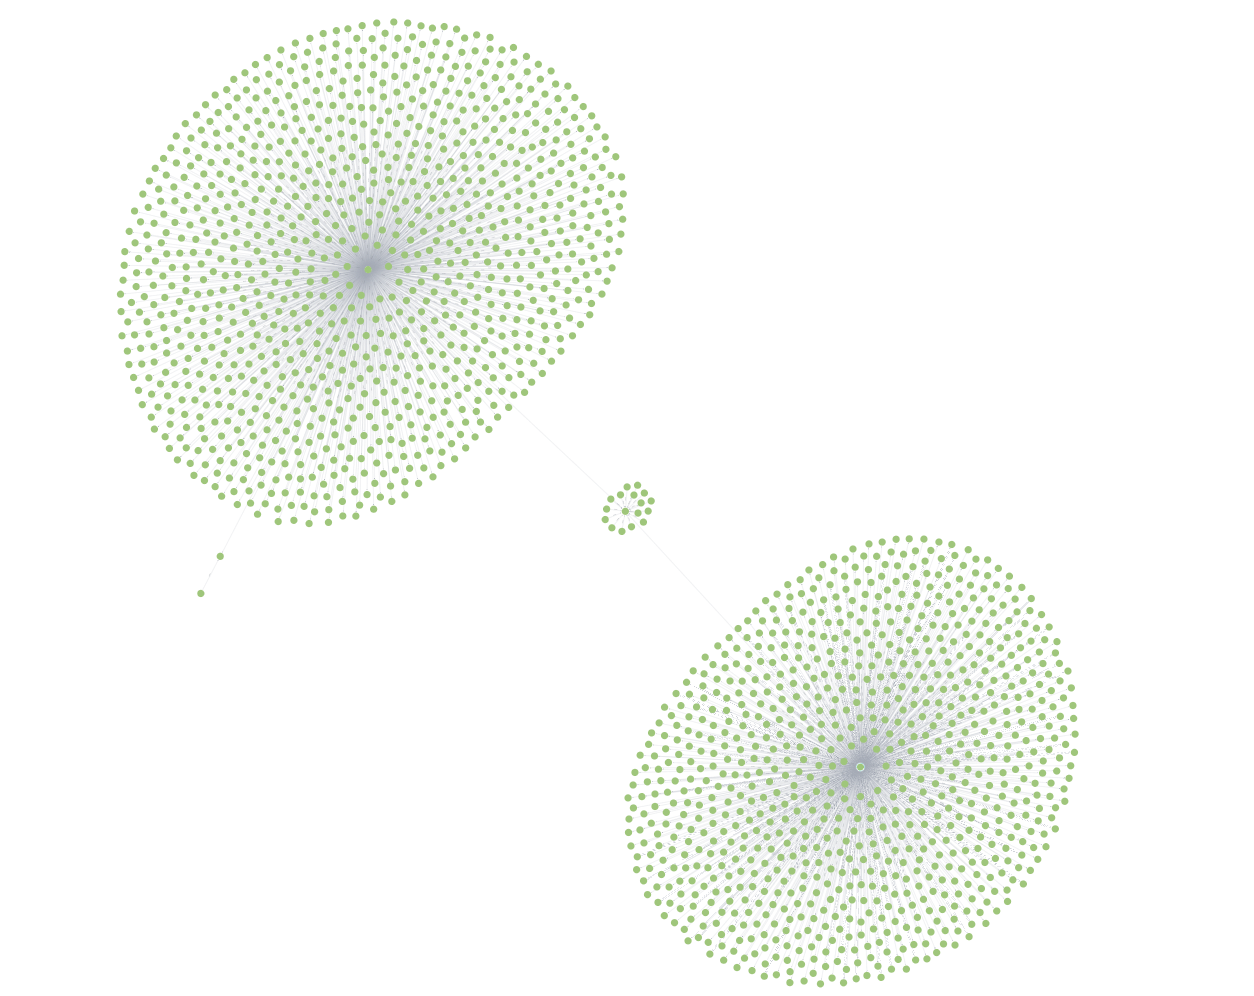
\includegraphics[width=0.8\textwidth]{../neo4j_query1_graph.png}
  \caption{Social network graph of the top 10 most-connected users. The two large clusters represent Walker's and Ruggy's friend networks.}
\end{figure}

There is no strong correlation between friend count and review count. Walker
leads with 14,995 friends but only 585 reviews --- highly social but not a
prolific reviewer. Conversely, Randy has the most reviews (3,315) with fewer
friends. Social connectivity and review activity are independent dimensions.
Mean star ratings cluster tightly (3.62--4.33), suggesting social influence
does not systematically bias rating behaviour.

\subsection{Query 2: Top 3 Businesses per State \marks{3}}

\begin{table}[H]
  \centering
  \footnotesize
  \setlength{\tabcolsep}{4pt}
  \begin{tabularx}{\textwidth}{llp{2.2cm}>{\raggedright\arraybackslash}Xrr}
    \toprule
    \textbf{St.} & \textbf{Business Name} & \textbf{City} & \textbf{Top Categories} & \textbf{Stars} & \textbf{Rev.} \\
    \midrule
    AZ & Let's Sweat                  & Tucson       & Yoga, Fitness, Cycling          & 5.00 & 59 \\
    AZ & Premier Pest Solutions       & Tucson       & Local Services, Pest Control    & 5.00 & 56 \\
    AZ & Tremendez Jewelry \& Repair  & Tucson       & Jewelry, Watch Repair           & 4.98 & 55 \\
    FL & AllVitae Health \& Chiro.    & Tampa        & Massage, Skin Care, Health Coach & 5.00 & 67 \\
    FL & Gerardo Luna Photographs     & Tampa        & Photography, Event Planning     & 4.98 & 51 \\
    FL & Tampa Bay Rum Company        & Tampa        & Food, Distilleries              & 4.96 & 57 \\
    IN & Alvin Lui                    & Indianapolis & Arts, Entertainment, Magicians  & 5.00 & 50 \\
    IN & Brick \& Mortar Barber Shop  & Indianapolis & Barbers, Beauty \& Spas         & 4.97 & 72 \\
    IN & kOMpose                      & Indianapolis & Life Coach, Yoga, Fitness       & 4.97 & 58 \\
    PA & Guldner's Collision Service  & Philadelphia & Automotive, Body Shops          & 5.00 & 57 \\
    PA & Campbell Jewelers            & Philadelphia & Jewelry, Jewelry Repair         & 5.00 & 55 \\
    PA & Sugar Bar Salon              & Philadelphia & Hair Removal, Beauty \& Spas    & 5.00 & 55 \\
    TN & Taylor Home Solutions        & Nashville    & Carpeting, Home Services, HVAC  & 5.00 & 50 \\
    TN & Music City Cats              & Nashville    & Pet Services, Dog Walkers       & 5.00 & 54 \\
    TN & Walls Jewelry Repairing      & Nashville    & Jewelry, Watch Repair           & 5.00 & 114 \\
    \bottomrule
  \end{tabularx}
  \caption{Top 3 businesses per state by average star rating ($\geq$50 reviews)}
\end{table}

All top businesses have near-perfect ratings (4.96--5.00) with modest review
counts (50--114), reflecting \textbf{statistical fragility} --- a small number
of very satisfied customers can maintain a perfect score. Category diversity
across states is notable: AZ favours wellness/fitness, FL hospitality and
food, IN entertainment/grooming, PA automotive/jewellery, TN home services.

\subsection{Query 3: Top 10 Users Across Most Distinct Cities \marks{3}}

All 10 users covered all 5 cities in the subset. Since the dataset was
subsetted to exactly 5 cities, 5 is the ceiling --- a dataset limitation, not
a meaningful differentiation. On the full Yelp dataset, this query would
effectively identify travelling reviewers and map food tourism patterns across
states.

The differentiator is \textbf{per-city mean rating variation}:
\begin{itemize}
  \item \textbf{David}: rates Tampa highly (4.50) but Indianapolis lower
    (3.60) --- possible preference for Tampa's business landscape.
  \item \textbf{Olivier}: rates Tucson at 4.00 but Indianapolis at 2.50 ---
    significant city-level bias.
  \item \textbf{S}: consistently generous rater (3.75--5.00 across all
    cities). Note: truncated name is a data quality issue in the Yelp source.
\end{itemize}

\subsection{Query 4: Category-Specific Rating Comparison --- Restaurants \marks{3}}

\begin{figure}[H]
  \centering
  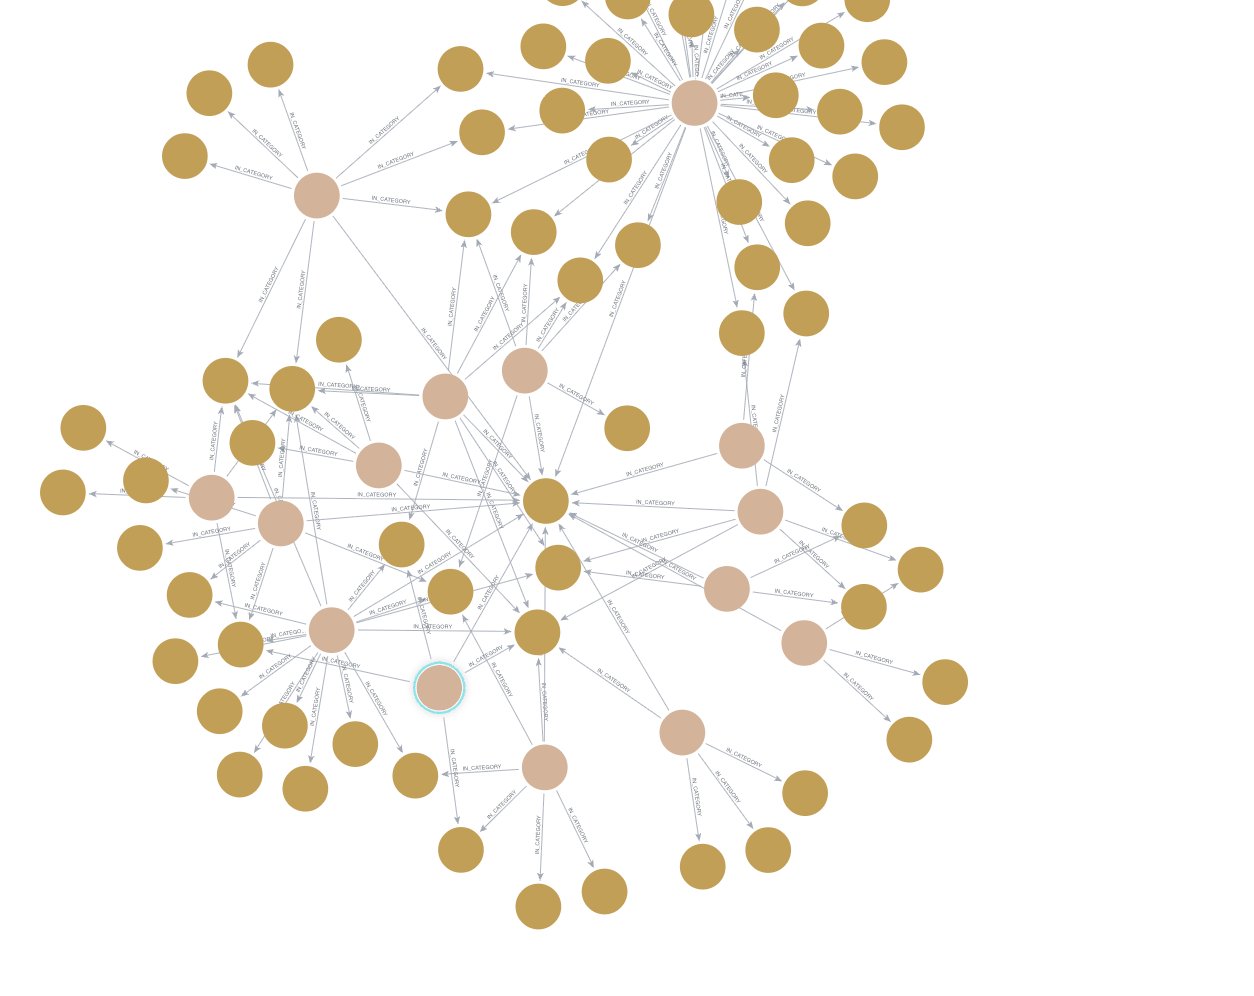
\includegraphics[width=0.85\textwidth]{../neo4j_query4_graph.png}
  \caption{User $\to$ Review $\to$ Business $\to$ Category traversal graph for the Restaurants category}
\end{figure}

\begin{table}[H]
  \centering
  \small
  \begin{tabular}{p{2cm}p{2.5cm}p{3cm}p{2.5cm}p{2cm}}
    \toprule
    \textbf{User} & \textbf{Restaurants Reviewed} & \textbf{User Avg (Restaurants)} & \textbf{User Overall Avg} & \textbf{Deviation} \\
    \midrule
    Michelle  & 714 & 4.01 & 4.08 & $-$0.07 \\
    Boon      & 631 & 3.90 & 3.89 & +0.01 \\
    Bill      & 608 & 4.05 & 4.07 & $-$0.02 \\
    Brett     & 556 & 4.19 & 4.24 & $-$0.05 \\
    michelle  & 547 & 3.85 & 3.88 & $-$0.03 \\
    Karen     & 538 & 3.53 & 3.62 & $-$0.10 \\
    \bottomrule
  \end{tabular}
  \caption{Users who reviewed $\geq$5 Restaurants, compared against their own overall average}
\end{table}

Most users rate restaurants \textbf{slightly lower} than their overall average
(largely negative deviations), indicating a more critical lens applied to food
specifically. \textbf{Karen} ($-$0.10) is the most category-critical.
\textbf{Boon} is the most consistent (+0.01). \textbf{Michelle} reviewed 714
restaurants --- an extreme power user --- yet her deviation is a modest
$-$0.07, suggesting her restaurant behaviour closely mirrors her general
reviewing style.

\subsection{Query 5: Reproducing MongoDB Query 1 in Cypher \marks{1}}

\begin{table}[H]
  \centering
  \begin{tabular}{lrrl}
    \toprule
    \textbf{City} & \textbf{Avg Stars} & \textbf{Total Reviews} & \textbf{Business Count} \\
    \midrule
    Philadelphia & 3.69 & 895,422 & 7,288 \\
    Indianapolis & 3.64 & 320,311 & 3,330 \\
    Nashville    & 3.64 & 416,408 & 3,414 \\
    Tampa        & 3.63 & 405,732 & 3,988 \\
    Tucson       & 3.58 & 352,978 & 3,963 \\
    \bottomrule
  \end{tabular}
\end{table}

\textbf{Results match closely}: rankings are identical (Philadelphia first,
Tucson last). Minor differences in total review counts (MongoDB: 863,550 vs.\
Cypher: 895,422 for Philadelphia) arise because MongoDB used the pre-stored
\code{review\_count} field on the business document, while Cypher counted
actual Review nodes present in the ingested graph subset.

\textbf{Which database is better suited?} MongoDB is better for this query.
It is a pure aggregation on a single collection --- no relationship traversal
is needed. The \code{\$match $\to$ \$group $\to$ \$sort} pipeline is highly
optimised for flat, tabular aggregations. Cypher must traverse
\code{(Business)<-[:REVIEWS]-(Review)} edges to count reviews, which is elegant
but slower for aggregate-only analytics. The graph model's strength shows when
queries need relationship traversal --- friend networks, multi-hop paths,
category recommendations --- not flat aggregations.

% ═════════════════════════════════════════════════════════════════════════════
\section*{Appendix: Query Scripts}
% ═════════════════════════════════════════════════════════════════════════════

All MongoDB queries are provided in \code{MongoDB\_Queries.txt}.\\
All Neo4j/Cypher queries are provided in \code{Neo4j\_Cypher\_Queries.txt}.

% ═════════════════════════════════════════════════════════════════════════════
\section*{AI Usage}
% ═════════════════════════════════════════════════════════════════════════════

Claude (Anthropic) was used to assist with schema design reasoning, query
writing, and report structuring. Full conversation log:\\
\url{https://claude.ai/share/dbff8110-f2ef-45b1-a294-e9bed37d1521}

\end{document}
